\section{構築したシステムの概要}
構築したシステムでは,人間が作成した
「次の角まで直進.左折.」などのシナリオから指示された道順に従い,カメラ画像に基づいて目的地まで自律移動する.
\figref{fig:abs}に構築したシステムの概要と自律移動の流れを示す.
構築したシステムは\\
1)シナリオを分解し,「条件」と「行動」を抽出するモジュール(以後,シナリオモジュールと呼ぶ)\\
2)カメラ画像と目標方向に基づいて,経路を追従するモジュール(以後,経路追従モジュールと呼ぶ)\\
3)カメラ画像を基に通路の特徴を分類するモジュール(以後,通路分類モジュールと呼ぶ)\\
% 〜で述べるシナリオモジュールと
% 〜で述べる経路追従モジュール
% 〜で述べる通路分類モジュールの
3つのモジュールで構成されている.
ロボットはaからdの一連の流れにより指示された道順に従って目的地まで自律移動する.
\vspace{3zh}
\begin{figure}[htbp]
    \centering
     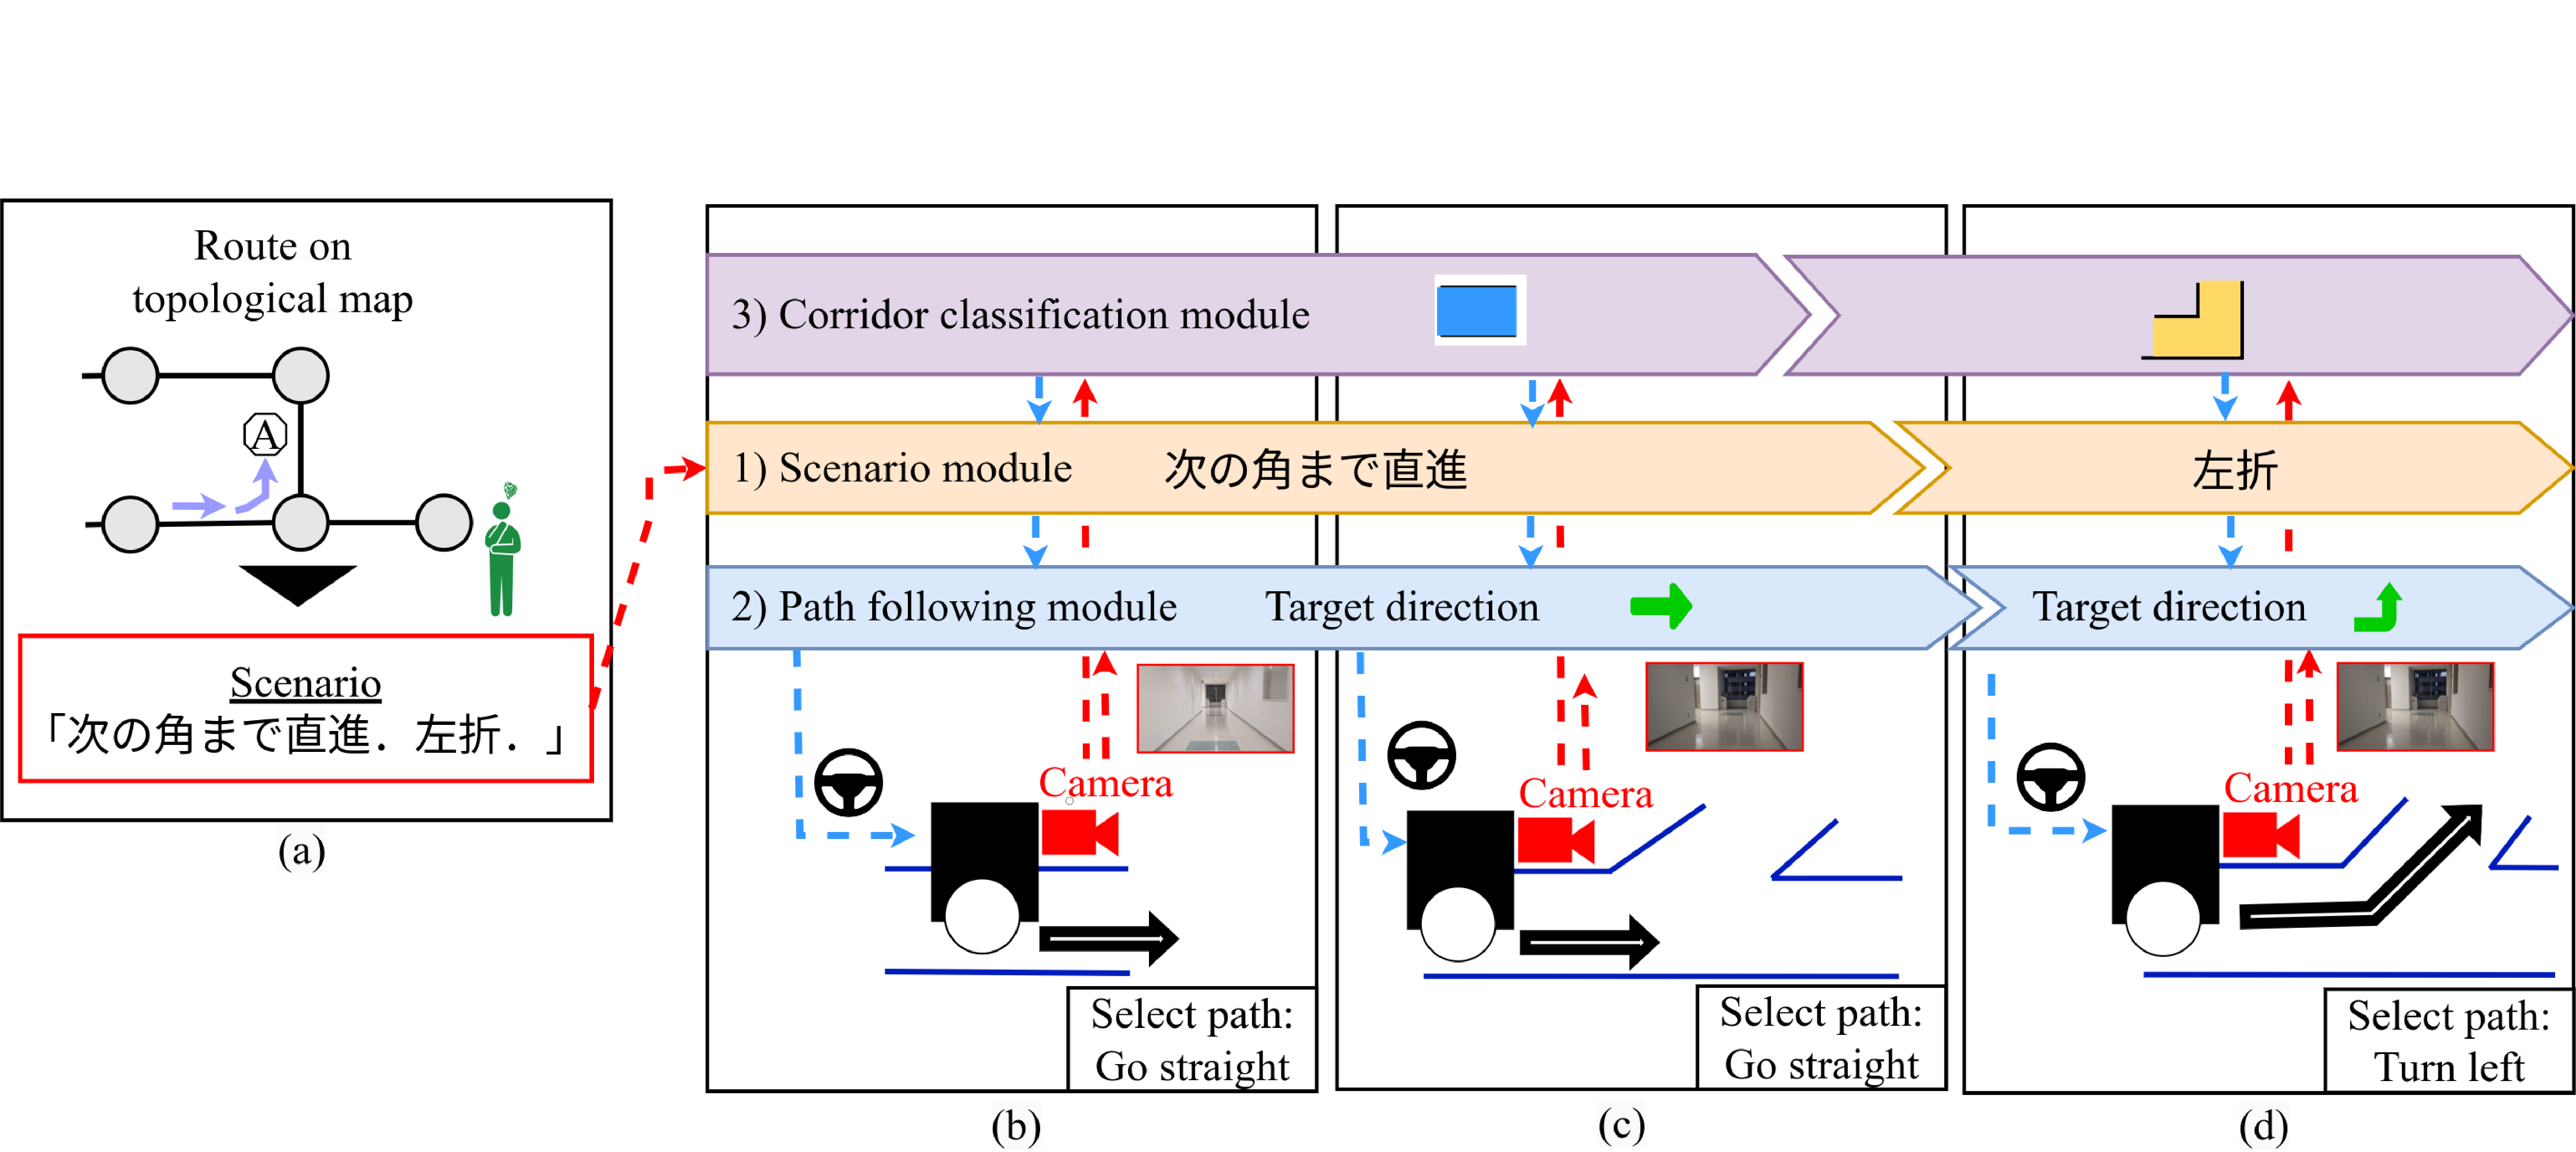
\includegraphics[width=130mm]{images/pdf/absv3.pdf}
     \caption{Overview of constructed system (Quoted from \cite{haruyama2023})}\label{fig:abs}
\end{figure}
\begin{enumerate}
    \item [(a)] トポロジカルマップ上の目的地に応じて,
    人間が「条件」と「行動」で構成されるシナリオを作成する.
    例えば,図のトポロジカルマップ上でAを目的地とするシナリオは「次の角まで直進.左折.」となる.
    \item [(b)] 作成したシナリオをシナリオモジュールへ入力する.
    シナリオモジュールは入力されたシナリオを分解し,「条件」と「行動」を抽出する.
    1つ目の条件と行動のセットは「次の角まで」と「直進」となる.
    この「直進」を目標方向として経路追従モジュールへ与える.
    経路追従モジュールは,カメラ画像と与えられた
    目標方向に基づいて,経路に沿って直進する.
    \item [(c)] ロボットが角に近づくと,
    % 通路分類モジュールの分類結果が角となり,
    通路分類モジュールがカメラ画像に基づいて
    通路を「角」と分類して,それをシナリオモジュールに与える.
    シナリオモジュールはそれを基に「次の角まで」という条件を満たしたかを判定する.
    この場合は条件を満たしているため,2つ目の行動である「左折」
    へ遷移する.
    \item [(d)]「左折」に基づいて,経路追従モジュールは
    経路に沿って角を左折する.
\end{enumerate}

% なお3つのモジュールはRobot Operating System(以下,ROS)\cite{ros}のフレームワーク上で作成している.
% また,通路分類モジュールと経路追従モジュールでは
% 機械学習のフレームワークとしてpytorch\cite{torch}を使用している
